\documentclass[tikz,border=3mm]{standalone}
\usepackage{amsmath,amssymb}
\usetikzlibrary{shapes.geometric, arrows.meta, positioning}

\begin{document}
\begin{tikzpicture}[
    auto,
    >=Stealth,
    node distance=0.75cm,
    font=\small\sffamily,
    stage/.style={draw=blue!80!black, fill=blue!6, rectangle, rounded corners=3pt,
                  text centered, minimum height=0.9cm, line width=0.8pt, inner sep=6pt},
    io/.style={draw=gray!70!black, fill=gray!12, rectangle, text centered, 
               minimum height=0.9cm, line width=0.8pt, inner sep=6pt},
    spill/.style={draw=teal!70!black, fill=teal!15, rectangle, rounded corners=3pt, 
                  text centered, font=\small\sffamily\bfseries, minimum height=0.75cm, line width=0.8pt, inner sep=5pt},
    reject/.style={draw=gray!60, fill=gray!20, rectangle, rounded corners=3pt, 
                   text centered, minimum height=0.75cm, line width=0.8pt, inner sep=5pt},
    arrow/.style={draw=black!80, ->, line width=0.8pt}
]
    \node [io] (input) {Raw SAR\\Image $I$};
    \node [stage, right=of input] (filter) {Speckle Filtering\\(Lee $7\times 7$, $L=4$)};
    \node [stage, right=of filter] (thresh) {Candidate Thresholding\\(Global Otsu $T^*$)};
    \node [stage, right=of thresh] (morph) {Morphology \& Area\\Pruning ($A \ge 64$ px)};
    \node [stage, right=of morph] (feat) {8-D Region Features\\$\mathbf{x}_i \in \mathbb{R}^8$};
    \node [stage, right=of feat] (clf) {Supervised Classifier\\(LinearSVM / CART)};
    
    \node [spill, above right=0.2cm and 0.8cm of clf] (out_spill) {Confirmed Oil Spill ($y_i=1$)};
    \node [reject, below right=0.2cm and 0.8cm of clf] (out_reject) {Rejected Dark Region ($y_i=0$)};

    \draw [arrow] (input) -- (filter);
    \draw [arrow] (filter) -- node[above, font=\scriptsize] {$I_f$} (thresh);
    \draw [arrow] (thresh) -- node[above, font=\scriptsize] {$B$} (morph);
    \draw [arrow] (morph) -- node[above, font=\scriptsize] {$\{\Omega_i\}$} (feat);
    \draw [arrow] (feat) -- node[above, font=\scriptsize] {$\mathbf{x}_i$} (clf);
    \draw [arrow] (clf) |- (out_spill);
    \draw [arrow] (clf) |- (out_reject);
\end{tikzpicture}
\end{document}
